\section{Introduktion}

Vores projekt tager udfordringen op med en mejetærsker (eller et andet køretøj), som har den problemstilling, at den kan komme ud i ujævnt terræn, hvormed at tanken på mejetærskeren kan få overbalance til den ene side og evt. tippe køretøjet eller tabe gods overbord. Ved at lave et system, som selv kan nivellere ”overkroppen” af køretøjet til vandret position, uanset ”underkroppens” vinkel, kan dette problem løses. Dette sikre at både kabinen og tanken på mejetærskeren altid vil være i vandret position vinkelret på køreretningen i ujævnt terræn.

\begin{figure}[H]
	\centering
	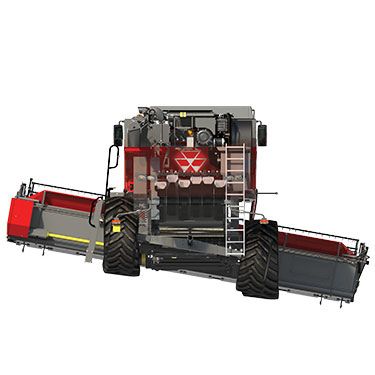
\includegraphics[width = 300pt]{figur/Visionbillede}
	\caption{Visionsbillede}
	\label{fig:konceptbillede}
\end{figure}

Kontrolsystemet kommer til at bestå med en motor, et gyroskop og en LEGO bil, hvor overdelen kan vippe sidelæns. Det forventes at systemet kan regulere en horisontal vinkel på op til ±30 grader tilbage til vandret i ”overdelen” ±1 grad. Systemet skal være adaptivt, idet mængden af gods/korn kan variere og dermed ændre belastningen på motoren.   \\ 

